\section{Sicherheit}
\label{sec:sicherheit_basics}

Peer-to-Peer bildet das Overlay-Netzwerk. Darunter liegt das Internet, welches die Infrastruktur für die Kommunikation bereitstellt. Da bei der Übertragung von Nachrichten über das Internet die Gefahr besteht, dass die Nachrichten abgefangen und mitgelesen werden können, ist es wichtig, dass die Kommunikation sicher ist. Die Nachrichten müssen über Verteilerknoten oder Access Points übertragen werden, die nicht vertrauenswürdig sind. Mittels Kryptografie kann die Vertraulichkeit, Integrität und Authentizität der Kommunikation gewährleistet werden \Parencite[S. 7]{Hellmann_IT-Sicherheit}.


\subsection{Vertraulichkeit}
\label{subsec:vertraulichkeit_basics}

Die Vertraulichkeit der Kommunikation wird durch Verschlüsselung gewährleistet. Man unterschiedet zwei Formen der Kryptografie: \textit{symmetrische} und \textit{asymmetrische} Kryptografie. Bei der \textit{symmetrischen} Kryptografie wird nur ein Schlüssel für die Verschlüsselung und Entschlüsselung verwendet. Der Sender der Nachricht verschlüsselt die Nachricht mit einem Schlüssel und sendet die nun verschlüsselte Nachricht an den Empfänger. Der Empfänger kann die Nachricht mit dem gleichen Schlüssel entschlüsseln. Dadurch kann ein Angreifer, der die Nachricht abfängt, diese nicht entschlüsseln, da er den Schlüssel nicht kennt. Abbildung \ref{fig:symmetrische_verschluesselung} zeigt den Ablauf der symmetrischen Verschlüsselung.

\begin{center}
    \captionsetup{type=figure}
    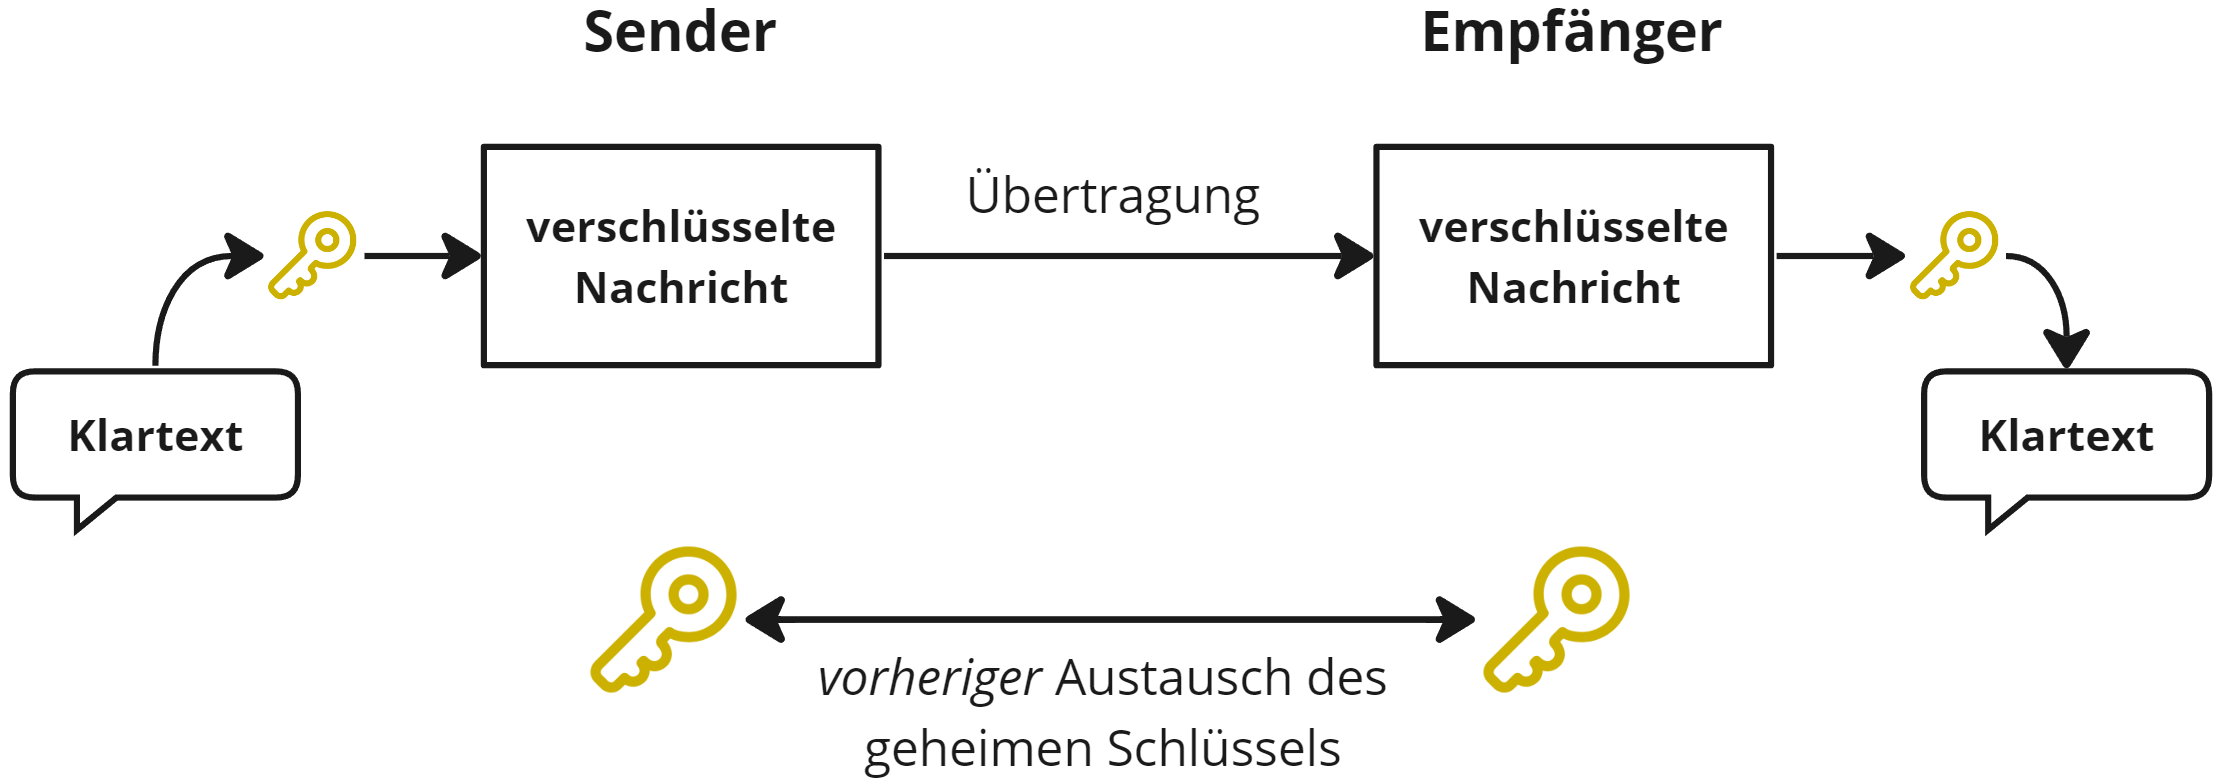
\includegraphics[width=1\linewidth]{images/symmetric_encryption.png}
    \caption{Symmetrische Verschlüsselung, in Anlehnung an \cite{ElektronikKompendium_symmetrischeVerschluesselung}}
    \label{fig:symmetrische_verschluesselung}
\end{center}

\noindent Das Problem bei der symmetrischen Kryptografie ist, dass der Schlüssel zu Beginn der Kommunikation vom Sender an den Empfänger gelangen muss. Dies stellt eine Herausforderung dar, wenn Sender und Empfänger sich noch nicht kennen und noch nie zuvor miteinander kommuniziert haben oder noch nicht über andere Wege einen Schlüssel ausgetauscht haben. Sollte der Schlüssel bei der Übertragung über einen unsicheren Kanal abgefangen werden, kann der Angreifer die Kommunikation entschlüsseln und somit mitlesen \Parencites[S. 644]{DiffieHellman_NewDirectionsInCryptography}[S. 5-8]{Wong_KryptoPraxis}. 

In diesem Fall kann eine Schlüsselvereinbarung verwendet werden, um einen gemeinsamen Schlüssel zu erhalten. Bei der Schlüsselvereinbarung wird ein Schlüssel zwischen zwei Parteien vereinbart, ohne dass dieser über einen unsicheren Kanal übertragen werden muss \Parencite[S. 102]{Wong_KryptoPraxis}. Abbildung \ref{fig:schluesselvereinbarung} zeigt den Ablauf der Schlüsselvereinbarung.

\begin{center}
    \captionsetup{type=figure}
    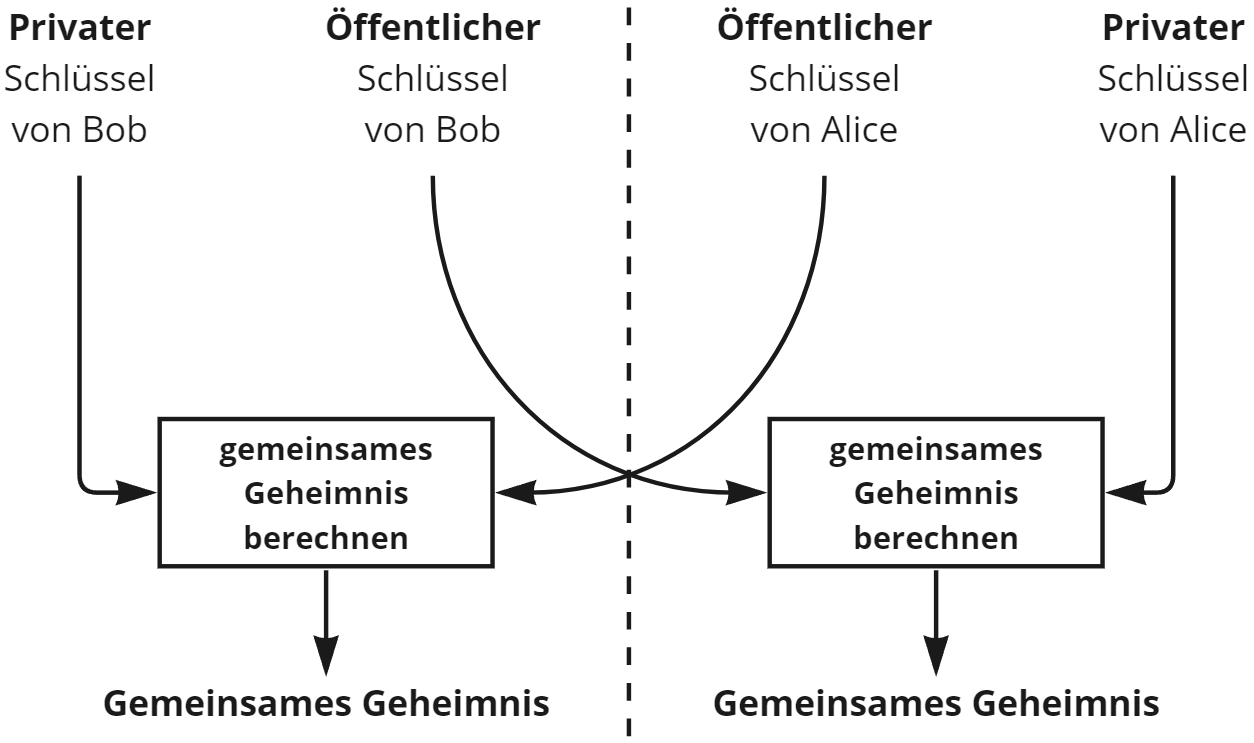
\includegraphics[width=0.7\linewidth]{images/key_exchange.png}
    \caption{Schlüsselvereinbarung, in Anlehnung an \cite[S. 102]{Wong_KryptoPraxis}}
    \label{fig:schluesselvereinbarung}
\end{center}

\noindent Beide Teilnehmer generieren einen privaten Schlüssel und einen öffentlichen Schlüssel. Durch die Kombination des öffentlichen Schlüssels des anderen Teilnehmers und des eigenen privaten Schlüssels wird ein gemeinsamer Schlüssel generiert. Dieser gemeinsame Schlüssel kann dann für die symmetrische Verschlüsselung verwendet werden \Parencite[S. 102]{Wong_KryptoPraxis}.


Bei der \textit{asymmetrische} Kryptografie (auch \textit{Public-Key-Kryptografie} genannt) wird anstatt nur eines Schlüssels ein Schlüsselpaar generiert, das aus einem öffentlichen und einem privaten Schlüssel besteht. Der öffentliche Schlüssel des Empfängers wird zum Verschlüsseln der Nachrichten verwendet und zum Entschlüsseln der Nachrichten wird der private Schlüssel des Empfängers verwendet. Der öffentliche Schlüssel des Empfängers kann von jedem verwendet werden, um Nachrichten an den Empfänger zu verschlüsseln. Nur der Empfänger kann die Nachrichten entschlüsseln, da nur er den privaten Schlüssel besitzt. Der Ablauf der asymmetrischen Verschlüsselung ist in Abbildung \ref{fig:asymmetrische_verschluesselung} dargestellt.


\begin{center}
    \captionsetup{type=figure}
    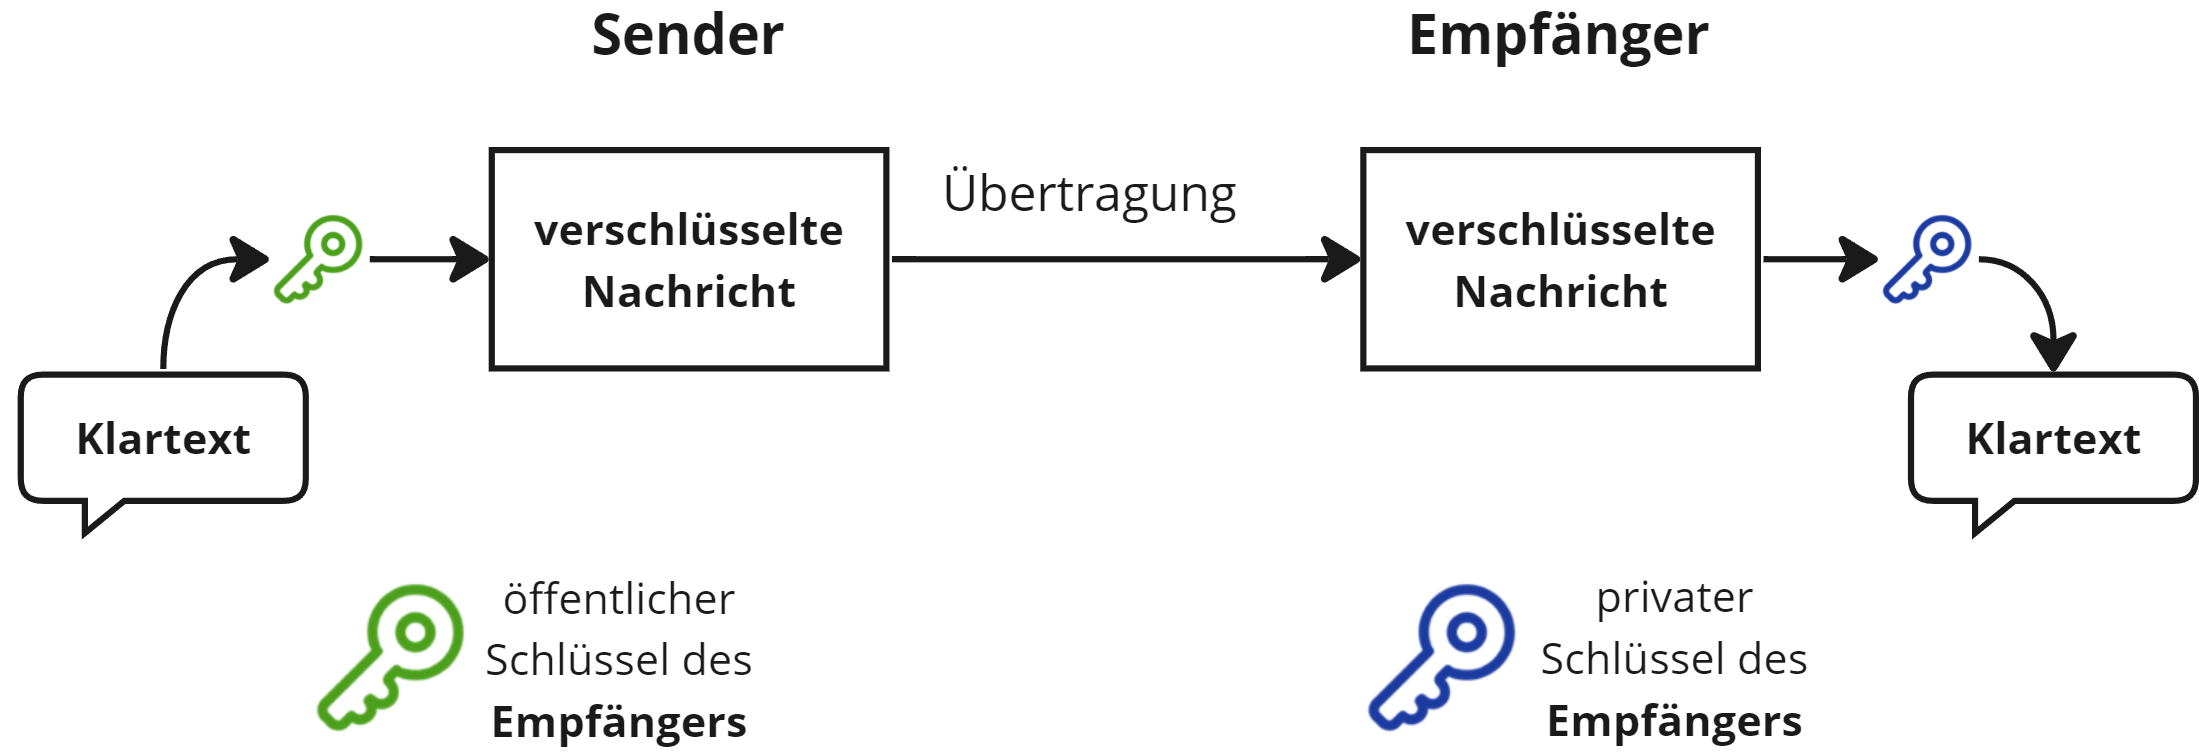
\includegraphics[width=1\linewidth]{images/asymmetric_encryption.png}
    \caption{Asymmetrische Verschlüsselung, in Anlehnung an \cite{ElektronikKompendium_asymmetrischeVerschluesselung}}
    \label{fig:asymmetrische_verschluesselung}
\end{center}

\noindent Es ist außerdem nicht möglich, Nachrichten, die mit dem öffentlichen Schlüssel verschlüsselt wurden, mit diesem auch wieder zu entschlüsseln \parencite{ElektronikKompendium_asymmetrischeVerschluesselung}. 

Diese beiden Verschlüsselungstechniken können kombiniert werden, um die Vorteile beider Verfahren zu nutzen. Der Schlüsselaustausch wird mit der asymmetrischen Verschlüsselung durchgeführt und die eigentliche Kommunikation wird mit der symmetrischen Verschlüsselung durchgeführt. Dadurch wird die Sicherheit der Kommunikation erhöht, da der Schlüssel nicht über einen unsicheren Kanal übertragen werden muss \Parencite[S. 5-8]{Wong_KryptoPraxis}. 


\subsection{Integrität}
\label{subsec:integritaet_signatur}

Um die Integrität der Kommunikation zu gewährleisten, werden digitale Signaturen verwendet. Um den Hash-Wert zu erhalten, wird die Nachricht mit einer Hashfunktion gehasht. Hashfunktionen sind Funktionen, die eine Eingabe beliebiger Länge in eine Ausgabe fester Länge umwandeln. Dabei ist es wichtig, dass die Hashfunktion zwei Eigenschaften erfüllt: \textit{Einwegfunktion} und \textit{Kollisionsresistenz}. Eine Einwegfunktion ist eine Funktion, die einfach zu berechnen ist, aber schwierig zu invertieren ist. Das bedeutet, dass es einfach ist, den Hash-Wert einer Nachricht zu berechnen, aber schwierig ist, die Nachricht aus dem Hash-Wert zu berechnen. Kollisionsresistenz bedeutet, dass es schwierig ist, zwei Nachrichten zu finden, die den gleichen Hash-Wert haben \parencite[S. 13-15]{Brünnler_BlockchainKurzGut}. Die folgende Abbildung zeigt, wie eine digitale Signatur funktioniert:

\begin{center}
    \captionsetup{type=figure}
    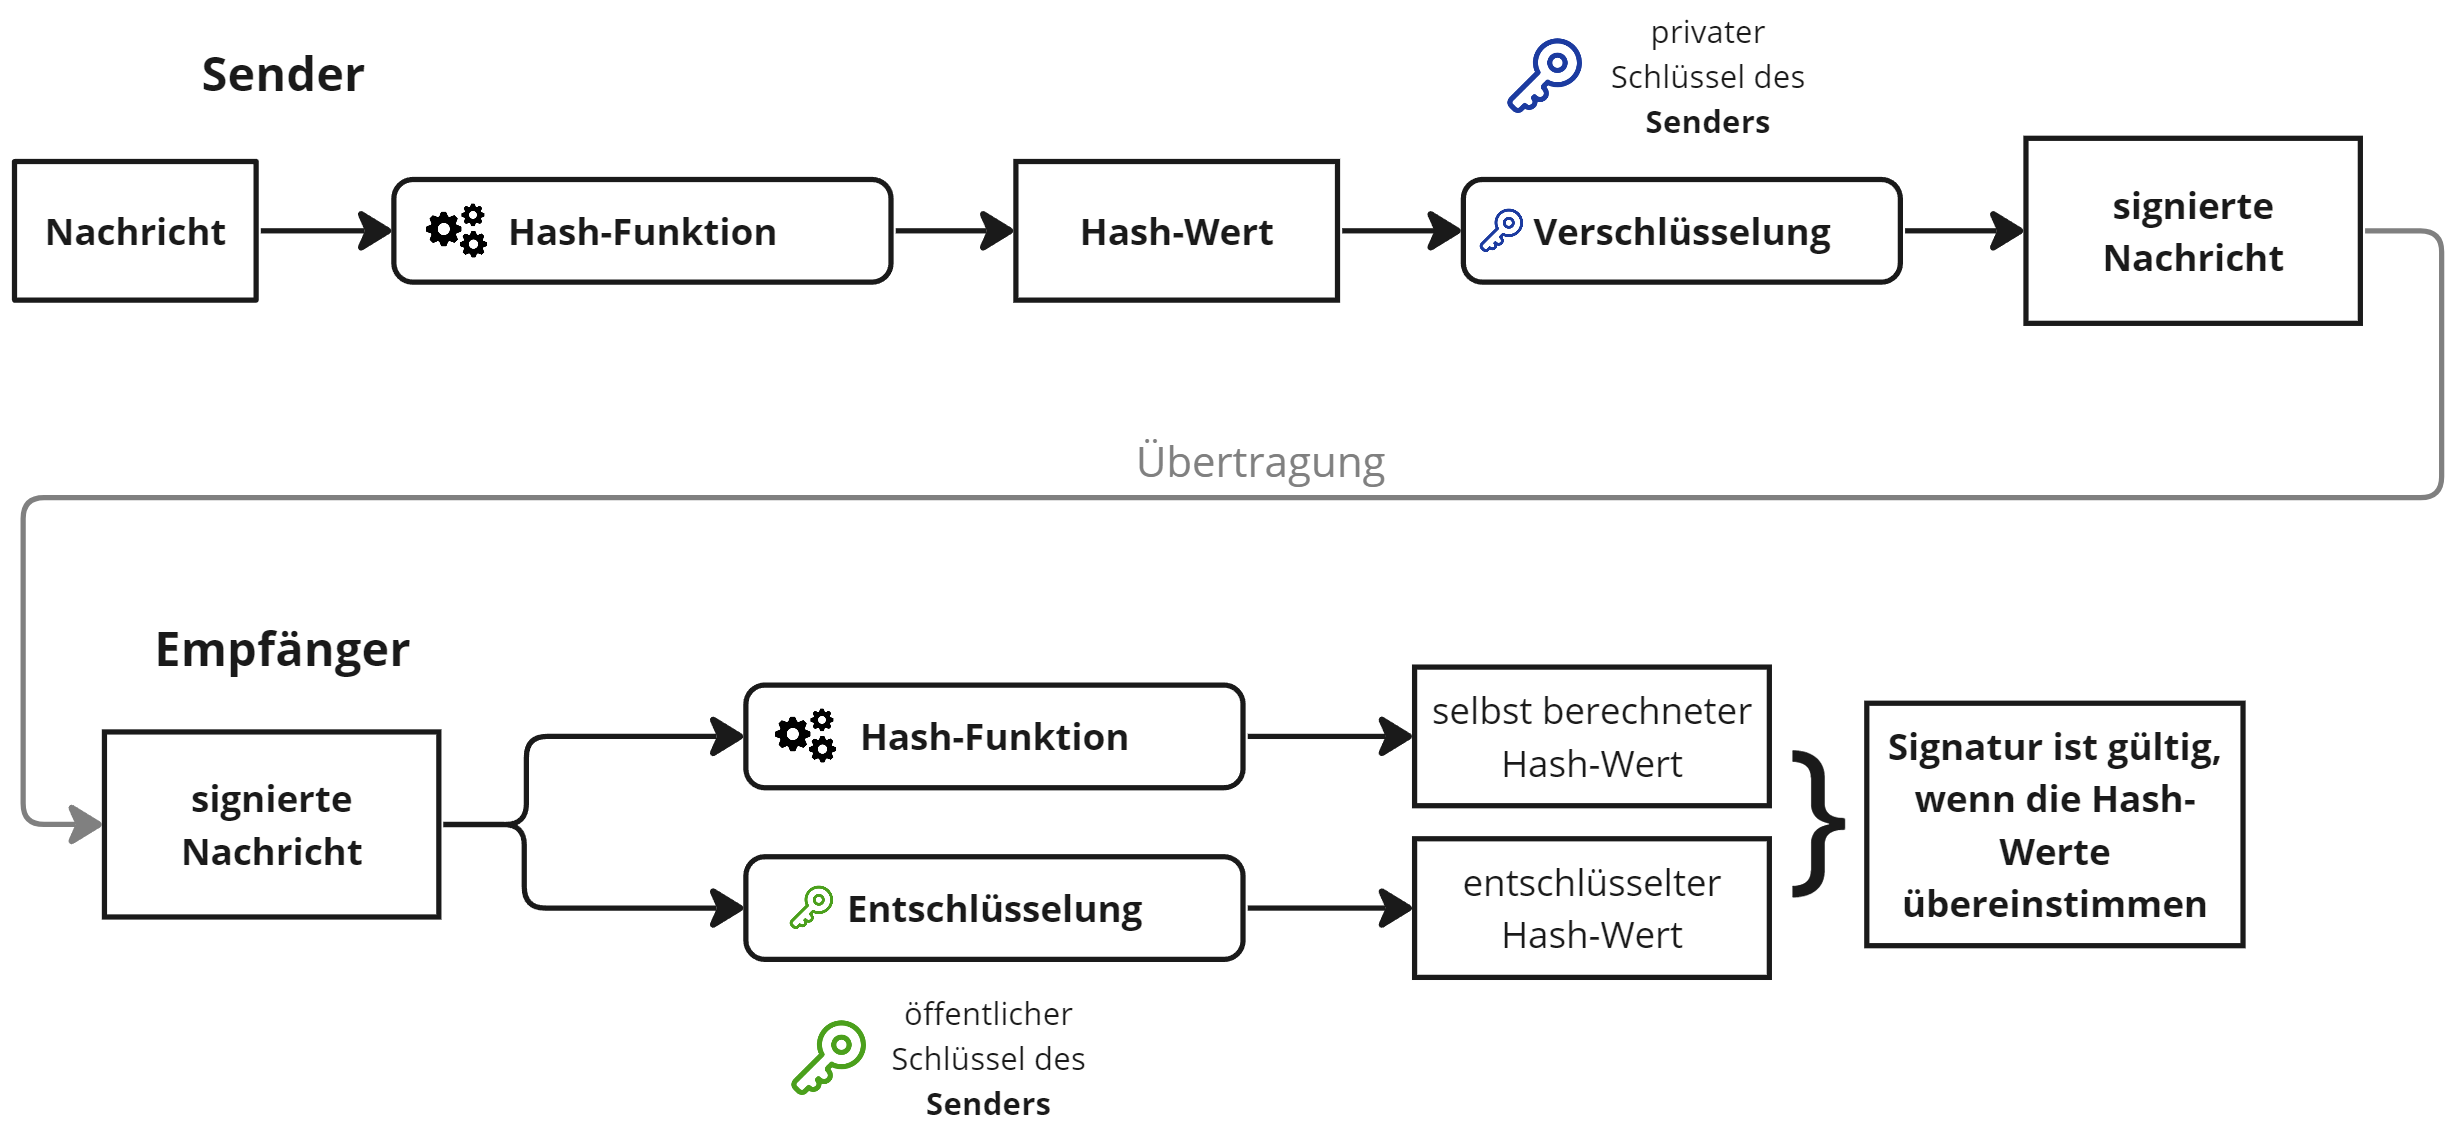
\includegraphics[width=1\linewidth]{images/signatur.png}
    \caption{Signatur, in Anlehnung an \cite{DocuSign_digitaleSignaturen}}
    \label{fig:signatur}
\end{center}

\noindent Der Sender berechnet den Hash-Wert der Nachricht, verschlüsselt diesen mit seinem privaten Schlüssel und hängt ihn (den Hash-Wert) an die Nachricht an. Der Empfänger entschlüsselt den Hash-Wert mit dem öffentlichen Schlüssel des Senders und berechnet den Hash-Wert der Nachricht selbst. Wenn der berechnete Hash-Wert mit dem entschlüsselten Hash-Wert übereinstimmt, kann der Empfänger sicher sein, dass die Nachricht nicht verändert wurde und somit die Integrität der Nachricht gewährleistet ist. Falls der berechnete Hash-Wert nicht mit dem entschlüsselten Hash-Wert übereinstimmt, wurde die Nachricht verändert und die Integrität der Nachricht ist nicht mehr gewährleistet \Parencite[S. 73-78]{Hellmann_IT-Sicherheit}. 


\subsection{Authentizität}

Für die Authentizität der Kommunikation werden ebenfalls Signaturen verwendet. Der Sender signiert die Nachricht mit seinem privaten Schlüssel und sendet die signierte Nachricht an den Empfänger. Durch die Integration der Blockchain in dieser Arbeit fungiert diese als öffentliches Verzeichnis oder auch Key-Server, in dem die öffentlichen Schlüssel der Teilnehmer gespeichert sind. Der Empfänger kann den öffentlichen Schlüssel des Senders aus der Blockchain auslesen, wodurch nachvollzogen werden kann, ob die Nachricht vom Sender stammt oder nicht.

\subsection{Ende-zu-Ende-Verschlüsselung am Beispiel des Signal-Protokolls}

Das Signal-Protokoll nutzt verschiedene fortschrittliche Verschlüsselungstechniken, um eine durchgängige Ende-zu-Ende-Verschlüsselung sicherzustellen. Für den Austausch von Schlüsseln bedient sich Signal des sogenannten \textit{Double Ratchet Algorithmus}. Der Double Ratchet Algorithmus ist eine kryptografische Methode, um Ende-zu-Ende-Verschlüsselung und \textit{Perfekte Zukunftssicherheit}, auch \textit{Perfect Forward Secrecy} genannt, zu ermöglichen. Dieser Algorithmus verwendet zwei Arten von Schlüsselpaaren: ein \textit{statisches} Schlüsselpaar, das für Authentifizierungszwecke dient, und ein \textit{flüchtiges} beziehungsweise \textit{ephemeres} Schlüsselpaar, das für die eigentliche Verschlüsselung der Nachrichten genutzt wird. Der Double Ratchet Algorithmus integriert zudem einen \textit{Root Key}, der für die Verschlüsselung der übermittelten Nachrichten verantwortlich ist und dessen Vereinbarung mittels Diffie-Hellman-Schlüsselaustausch erfolgt. Nach der Vereinbarung des Root Keys wird dieser genutzt, um einen \textit{Chain Key} zu generieren. Der Chain Key wiederum wird dazu verwendet, einen \textit{Message Key} zu erzeugen, welcher die eigentliche Verschlüsselung der Nachrichten ermöglicht. Das Kernelement dieses Algorithmus ist das \textit{Key Ratcheting}. Der Chain Key wird nach dem Empfang jeder Nachricht aktualisiert, indem er mittels erneutem Diffie-Hellman-Schlüsselaustausch und dem Root Key neu berechnet wird. Gleichzeitig wird der Message Key nach jeder übermittelten Nachricht aktualisiert, indem er durch erneuten Diffie-Hellman-Schlüsselaustausch und unter Einbeziehung des Chain Keys neu generiert wird. Dadurch wird sichergestellt, dass jeder Message Key nur einmal verwendet wird und somit die \textit{Perfekte Zukunftssicherheit} gewährleistet ist. Die \textit{Perfekte Zukunftssicherheit} bedeutet, dass selbst wenn ein Angreifer in der Zukunft den privaten Schlüssel eines Teilnehmers erlangt, er nicht in der Lage ist, die Kommunikation der Vergangenheit zu entschlüsseln \Parencite{Signal_DoubleRatchet}.
